\section{Задание 2. Приведение уравнения поверхности 2-го порядка к каноническому виду.}
\textbf{Условие.}

Дано уравнение поверхности 2-го порядка:

\[2x^2 + 4y^2 + 2z^2 + 2xz -12 = 0\]

План:
\begin{enumerate}
    \item С помощью теории квадратичных форм приведите к каноническому виду данное уравнение.
    \item Изобразите график уравнения в исходной системе координат.
Какую поверхность оно задаёт? Укажите на графике оси исходной и приведённой систем координат.
\end{enumerate}

\vspace{10mm}
\textbf{Решение.}

\begin{enumerate}
	\item Возьмем матрицу этой поверхности $Q(x,y,z) = 2x^2 + 4y^2 + 2z^2 + 2xz - 12 = a_{11}x^2 + 2a_{12}xy + a_{22}y^2 + 2a_{13}xz + 2a_{23}yz + a_{33}z^2 + C \Rightarrow Q_e = \begin{pmatrix} 2 & 0 & 1 \\ 0 & 4 & 0 \\ 1 & 0 & 2 \end{pmatrix}$. 
Чтобы привести ее к каноническому виду, найдем собственные числа этой матрицы: $|Q_e - \lambda E| = \begin{vmatrix} 2 - \lambda & 0 & 1 \\ 0 & 4 - \lambda & 0 \\ 1 & 0 & 2 - \lambda  \end{vmatrix} = 0.$ Раскроем определитель по второй строчке: $(4 - \lambda) \begin{vmatrix} 2 - \lambda & 1 \\ 1 & 2 - \lambda \end{vmatrix} = (4 - \lambda)( (2 - \lambda)^2 - 1) = (4 - \lambda)(\lambda^2 -4\lambda + 3) = (4 - \lambda)(3 - \lambda)(1 - \lambda) = 0 \Rightarrow \lambda_1 = 4, \lambda_2 = 3, \lambda_3 = 1.$ \\
Тогда матрица этой поверхности в каноническом виде будет выглядеть так: $\begin{pmatrix} 4 & 0 & 0 \\ 0 & 3 & 0 \\ 0 & 0 & 1 \end{pmatrix}$. Проверим правильность с помощью преобразования координат. Собственные векторы этой матрицы: 
$Q_e x_1 = \lambda_1 x_1 \Rightarrow \begin{pmatrix} 2 & 0 & 1 \\ 0 & 4 & 0\\ 1 & 0 & 2 \end{pmatrix} \begin{pmatrix} a_1 \\ a_2 \\ a_3 \end{pmatrix} = \begin{pmatrix} 4a_1 \\ 4a_2 \\ 4a_3 \end{pmatrix}  \Rightarrow 2a_1 = a_3, a_2 = a_2, 2a_3 = a_1 \Rightarrow x_1 = C\begin{pmatrix} 0 \\ 1 \\ 0 \end{pmatrix};$
$Q_e x_2 = \lambda_2 x_2 \Rightarrow \begin{pmatrix} 2 & 0 & 1 \\ 0 & 4 & 0\\ 1 & 0 & 2 \end{pmatrix} \begin{pmatrix} a_1 \\ a_2 \\ a_3 \end{pmatrix} = \begin{pmatrix} 3a_1 \\ 3a_2 \\ 3a_3 \end{pmatrix}  \Rightarrow a_1 = a_3, a_2 = 0 \Rightarrow x_2 = C\begin{pmatrix} 1 \\ 0 \\ 1 \end{pmatrix};$
$Q_e x_3 = \lambda_3 x_3 \Rightarrow \begin{pmatrix} 2 & 0 & 1 \\ 0 & 4 & 0\\ 1 & 0 & 2 \end{pmatrix} \begin{pmatrix} a_1 \\ a_2 \\ a_3 \end{pmatrix} = \begin{pmatrix} a_1 \\ a_2 \\ a_3 \end{pmatrix}  \Rightarrow a_1 = -a_3, a_2 = 0 \Rightarrow x_3 = C\begin{pmatrix} 1 \\ 0 \\ -1 \end{pmatrix}.$ \\
Тогда ортонормированный базис из их этих векторов: $\begin{pmatrix} 0 & 1 & 0 \\ \frac{1}{\sqrt{2}} & 0 & \frac{1}{\sqrt{2}} \\ \frac{1}{\sqrt{2}} & 0 & -\frac{1}{\sqrt{2}}\end{pmatrix}$, преобразование координат:  $\begin{pmatrix} 0 & 1 & 0 \\ \frac{1}{\sqrt{2}} & 0 & \frac{1}{\sqrt{2}} \\ \frac{1}{\sqrt{2}} & 0 & -\frac{1}{\sqrt{2}}\end{pmatrix}$ $\begin{pmatrix} 2 & 0 & 1 \\ 0 & 4 & 0 \\ 1 & 0 & 2 \end{pmatrix}$ $\begin{pmatrix} 0 & \frac{1}{\sqrt{2}} & \frac{1}{\sqrt{2}} \\ 1 & 0 & 0 \\ 0 & \frac{1}{\sqrt{2}} & -\frac{1}{\sqrt{2}}\end{pmatrix} = \begin{pmatrix} 4 & 0 & 0 \\ 0 & 3 & 0 \\ 0 & 0 & 1 \end{pmatrix}$.\\

Тогда уравнение будет $Q(x,y,z) = 4x^2 + 3y^2 + z^2 - 12$, канонический вид уравнения: $\frac{x^2}{3} + \frac{y^2}{4} + \frac{z^2}{12} = 1$.
	\item Поверхность с осями исходной СО (черным цветом) и приведённой СО (разными цветами) 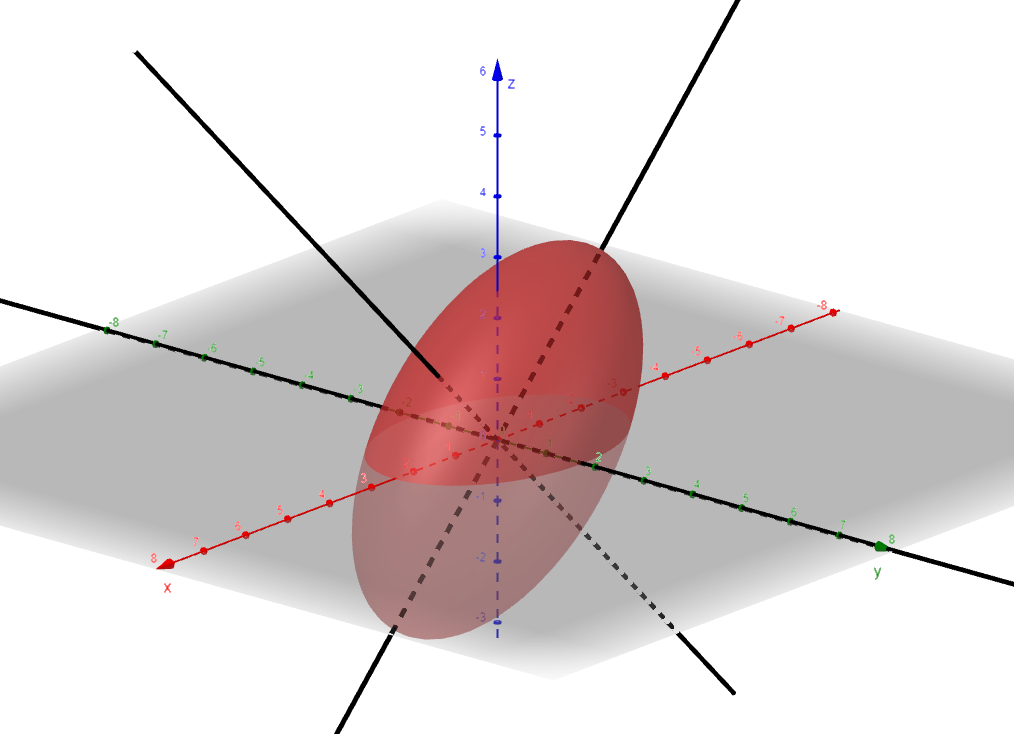
\includegraphics[scale=0.5]{images/2_2} \\
Уравнение задает эллипс.

\end{enumerate} 
